% !TeX program = pdflatex
\documentclass[10pt]{beamer}

\usepackage{amsmath, amssymb}
\usepackage{tikz}
\usetikzlibrary{arrows.meta,positioning,calc,decorations.pathreplacing}
\usepackage{multirow}
\usepackage{array}
\usepackage{booktabs}
\usepackage{makecell}
\usepackage{bm}
\usepackage[most]{tcolorbox}
\usepackage{soul}
\usefonttheme{professionalfonts}
\setbeamertemplate{navigation symbols}{}
\addtobeamertemplate{frametitle}{}{\vspace*{0.5cm}}
\setbeamertemplate{itemize item}{\usebeamercolor[fg]{frametitle}\small$\bullet$}
\setbeamertemplate{itemize subitem}{\usebeamercolor[fg]{frametitle}\scriptsize$\blacktriangleright$}
\setbeamertemplate{enumerate item}{\usebeamercolor[fg]{frametitle}\insertenumlabel.}

% --- Rounded blocks matching the reference slide style ---
\definecolor{llxBlockBlue}{RGB}{57,57,180}
\definecolor{llxBlockTitleBg}{RGB}{214,214,242}
\definecolor{llxBlockBodyBg}{RGB}{239,239,250}
\setbeamertemplate{blocks}[rounded][shadow=true]
\setbeamercolor{block title}{fg=llxBlockBlue,bg=llxBlockTitleBg}
\setbeamercolor{block body}{fg=black,bg=llxBlockBodyBg}
\setbeamerfont{block title}{size=\normalsize,series=\bfseries}

% --- page number ---
\setbeamertemplate{footline}{%
	\raisebox{10pt}{\makebox[\paperwidth]{\hfill\makebox[7em]{\normalsize\texttt{\insertframenumber/\inserttotalframenumber}}}}%
}

\setbeamerfont{footnote}{size=\scriptsize}
\renewcommand{\footnoterule}{\vspace{1pt}\hrule width 0.3\linewidth\vspace{2pt}}

% Outline with the current section highlighted (style of J. Hu's slides).
\definecolor{outlinegray}{gray}{0.72}
\newcommand{\outlineitem}[3]{%
  \ifnum\value{section}=0\relax\item[\textbf{#2.}]\textbf{#3}%
  \else\ifnum\value{section}=#1\relax\item[\textbf{#2.}]\textbf{#3}%
  \else\item[{\color{outlinegray}\textbf{#2.}}]{\color{outlinegray}#3}\fi\fi}
\newcommand{\outlinelist}{%
\begin{enumerate}\setlength{\itemsep}{10pt}
    \outlineitem{1}{I}{Introduction: Nonsmooth Composite Optimization}
    \outlineitem{2}{II}{Methodology: Fixed-Penalty Linearized ALM as GDA}
    \outlineitem{3}{III}{Results: Lower Bounds for Linearized Regularized ALMs}
    \outlineitem{4}{IV}{Open Discussion: Acceleration}
\end{enumerate}}
\AtBeginSection[]{%
    \begin{frame}[plain,noframenumbering]{Outline}
    \vspace{0.6cm}
    \outlinelist
    \end{frame}%
}

\newcommand{\red}[1]{{\color[rgb]{1,0,0}{#1}}}
\newcommand{\blue}[1]{{\usebeamercolor[fg]{frametitle}#1}}
\definecolor{okgreen}{RGB}{0,130,60}
\newcommand{\green}[1]{{\color{okgreen}{#1}}}
\definecolor{kktorange}{RGB}{200,90,0}
\newcommand{\orange}[1]{{\color{kktorange}{#1}}}
\newcommand{\titleblue}[1]{{\usebeamercolor[fg]{frametitle}#1}}
\newcommand{\citeb}[1]{{\color{gray!75!black}\footnotesize[#1]}}
% full reference at the bottom of the page, without a footnote number
\makeatletter
\usepackage{etoolbox}
\pretocmd{\beamer@checkframetitle}{\setcounter{footnote}{0}}{}{}
\makeatother

% --- notation (matches the manuscript) ---
\newcommand{\RR}{\mathbb{R}}
\newcommand{\bx}{\mathbf{x}}
\newcommand{\by}{\mathbf{y}}
\newcommand{\bz}{\mathbf{z}}
\newcommand{\bq}{\mathbf{q}}
\newcommand{\bmu}{\bm{\mu}}
\newcommand{\blmbd}{\bm{\lambda}}
\newcommand{\zero}{\mathbf{0}}
\newcommand{\calA}{\mathcal{A}}
\newcommand{\calD}{\mathcal{D}}
\newcommand{\calP}{\mathcal{P}}
\newcommand{\calL}{\mathcal{L}}
\newcommand{\calC}{\mathcal{C}}
\newcommand{\calG}{\mathcal{G}}
\newcommand{\prox}{\operatorname{prox}}

\title{Dual-Regularized ALM with a Fixed Penalty}
\subtitle{How Much Regularization Is Needed, and How Can We Accelerate?}
\author{Luxuan Li (Beihang University)\\[6pt]
{\small Joint work with}\\[1pt]
{\footnotesize Prof.\ Kangkang Deng (National University of Defense Technology)}\\
{\footnotesize Prof.\ Chunfeng Cui (Beihang University)}\\
{\footnotesize Prof.\ Jiang Hu (Tsinghua University)}}
\date{Vienna, November 6, 2026}

\begin{document}

\begin{frame}[noframenumbering,plain]
\titlepage
\end{frame}

% ---------------------------------------------------------------------
% Slide 1: Outline
\begin{frame}[plain,noframenumbering]{Outline}
\vspace{0.6cm}
\outlinelist
\end{frame}

% =====================================================================
\section{Introduction}
% =====================================================================

% ---------------------------------------------------------------------
% Slide 2: Problem
\begin{frame}{Problem}
\small
\begin{itemize}\setlength{\itemsep}{4pt}
    \item Consider the nonconvex composite problem
    \[
        \min_{\bx\in\RR^n}\ F(\bx):=f(\bx)+h(\calA(\bx))
        \tag{P}
    \]
    \item \textbf{Assumptions:}
    \begin{itemize}\setlength{\itemsep}{0pt}
        \item $f:\RR^n\to\RR$ is $L_f$-smooth, $G_f$-Lipschitz;
        \item $\calA:\RR^n\to\RR^m$ is $L_{\calA}$-smooth, $G_{\calA}$-Lipschitz;
        \item $h:\RR^m\to\RR$ is convex, $L_h$-Lipschitz, with a tractable $\prox_{th}$.
    \end{itemize}
    \item \textbf{Applications:} robust phase retrieval \citeb{Duchi '19}, CVaR \citeb{Mehta '23}, worst-group \citeb{Kirichenko '23}.
    \item \textbf{Our focus:} given $\epsilon>0$, the (iteration) complexity of first-order methods to find an $\epsilon$-KKT point.
\end{itemize}
% \textbf{Difficulty.} $\prox_h$ is easy, but $\prox_{h\circ\calA}$ is in general not available.
\end{frame}

% ---------------------------------------------------------------------
% Slide 3: How to handle the nonsmooth term
\begin{frame}{Handling the Nonsmooth Composition $h\circ\calA$}
\small
\red{\textbf{Core difficulty:}} $\prox_{th}$ is tractable, but $\prox_{t(h\circ\calA)}$ \red{is not}.

\vspace{0.25cm}
\begin{itemize}\setlength{\itemsep}{8pt}
    \item \textbf{Subgradient methods:} $\bx^{k+1}=\bx^k-\eta_k\mathbf g^k$ with $\mathbf g^k\in\partial F(\bx^k)$.
    \citeb{Bolte et al.\ '07; Davis--Drusvyatskiy '19; Li--Pan '26}
    \item \textbf{Prox-linear methods:} linearize $\calA$ inside $h\bigl(\calA(\bx^k)+J_{\calA}(\bx^k)(\bx-\bx^k)\bigr)$ and minimize a convex composite model per step.
    \citeb{Lewis--Wright '16; Drusvyatskiy--Paquette '19; Zhu--Li '26}
    \item \textbf{Variable smoothing:} replace $h$ by its Moreau envelope $M_h^t$ with $t\downarrow 0$.
    \citeb{Nesterov '05; B\"ohm--Wright '21; Beck--Rosset '23; Peng et al.\ '23}
    \item \blue{\textbf{Primal-dual methods:}} decouple $h$ and $\calA$ via $\by=\calA(\bx)$ and multiplier $\blmbd$, evaluating $h$ through $\prox_{th}$.
    \citeb{Bo\c{t}--Nguyen '20; Hallak--Teboulle '23; Deng et al.\ '25}
\end{itemize}
\end{frame}
% ---------------------------------------------------------------------
% Slide 4: Linearized ALM and epsilon-KKT points
\begin{frame}{Linearized Augmented Lagrangian Method}
\small

\begin{itemize}
\item Augmented Lagrangian of the split Problem~(P) with penalty $\rho>0$:
    \[
\calL_\rho(\bx,\by,\blmbd)=f(\bx)+h(\by)+\langle\blmbd,\calA(\bx)-\by\rangle+\tfrac{\rho}{2}\|\calA(\bx)-\by\|^2 .
    \]
    \item Single-loop scheme: linearized ALM:
    \[
        \begin{aligned}
            \bx^{k+1}&=\bx^k-\red{\eta}\,\nabla_{\bx}\calL_\rho\bigl(\bx^k,\by(\bx^k,\blmbd^k),\blmbd^k\bigr),\qquad 0<\red{\eta}\le 1/L_{\bx}(\red{\rho}),\\
            \by^{k+1}&=\by(\bx^{k+1},\blmbd^k),\qquad \by(\bx,\blmbd):=\prox_{\red{h/\rho}}\bigl(\calA(\bx)+\blmbd/\rho\bigr),\\
            \blmbd^{k+1}&=\blmbd^k+\rho\bigl(\calA(\bx^{k+1})-\by^{k+1}\bigr).
        \end{aligned}
    \]
    \item $\epsilon$-KKT point ($\epsilon>0$): $\bx\in\RR^n$ with $(\by,\bq)\in\RR^m\times\partial h(\by)$ such that
    \[
        \mathcal R_{\mathrm{KKT}}(\bx,\by,\bq):=\max\bigl\{\|\nabla f(\bx)+J_{\calA}(\bx)^\top\bq\|,\ \|\calA(\bx)-\by\|\bigr\}\le\epsilon .
    \]
\end{itemize}

\vspace{0.2cm}
\blue{\textbf{Limitation:}} $\rho$ enters both the primal stepsize $\eta\le 1/L_{\bx}(\rho)$ and the feasibility residual $\|\calA(\bx)-\by\|$.

\end{frame}

% ---------------------------------------------------------------------
% Slide 6: Existing ALMs and the penalty
\begin{frame}
\frametitle<1>{Existing Nonconvex ALMs: Large Penalty}
\frametitle<2>{From Large Penalty to Fixed-Penalty Linearized ALM}
\small
{\centering
\footnotesize
\renewcommand{\arraystretch}{1.0}
\setlength{\tabcolsep}{8pt}
\begin{tabular}{@{}cccc@{}}
\multicolumn{4}{@{}c@{}}{\textbf{Table 1.} Iteration complexity of existing nonconvex ALMs for finding $\epsilon$-KKT points.}\\
\toprule
Method & Loop & Penalty $\rho$ & Iteration complexity \\
\midrule
\makecell{Inexact ALM\\ \citeb{Sahin et al.\ '19}} & double & increasing & $\widetilde{\mathcal O}(\epsilon^{-4})$ \\
\makecell{Inexact ALM\\ \citeb{Li et al.\ '21}} & triple & increasing & $\widetilde{\mathcal O}(\epsilon^{-3})$ \\
\makecell{Linearized ALM\\ \citeb{Lu '22}} & \red{single} & \red{$\Theta(\epsilon^{-1})$} & \red{$\mathcal O(\epsilon^{-3})$} \\
\bottomrule
\end{tabular}\par}

\vspace{0.3cm}
\[
    \blue{\text{Feasibility:}}\quad
    \|\calA(\bx^{k+1})-\by^{k+1}\|\le\frac{2L_h}{\rho}=\epsilon
    \quad\implies\quad
    \red{\rho=2L_h/\epsilon}.
\]
\[
    \blue{\text{Iteration complexity:}}\quad
    \red{L_{\bx}(\rho)=\Theta(\rho)=\Theta(\epsilon^{-1})}
    \quad\implies\quad
    \mathcal O\Bigl(\frac{L_{\bx}(\rho)\,\Delta}{\epsilon^{2}}\Bigr)=\red{\mathcal O(\epsilon^{-3})}.
\]

\vspace{0.2cm}
\begin{overprint}
\onslide<1>
\blue{\textbf{Trade-off:}} For an $\epsilon$-KKT point, $\epsilon$-feasibility requires increasing $\red{\rho}$ to $\red{\Theta(\epsilon^{-1})}$, leading to $\red{\mathcal O(\epsilon^{-3})}$ complexity.
\onslide<2>
% \vspace{0.2cm}
\begin{block}{Motivating Question}
\centering
Can a \emph{fixed-penalty} linearized ALM, i.e.,\ with ${\rho=\Theta(1)}$ independent of $\epsilon$, still reach $\mathcal O(\epsilon^{-3})$ complexity?
\end{block}
\end{overprint}
\end{frame}

% =====================================================================
\section{Linearized ALM as GDA}
% =====================================================================

% ---------------------------------------------------------------------
% Slide 6: Problem (P) as a minimax problem
\begin{frame}{Problem~(P) as a Minimax Problem}
\small
\begin{itemize}\setlength{\itemsep}{2pt}
    \item Minimizing $\calL_\rho$ over $\by$ gives the \titleblue{reduced augmented Lagrangian}
    \[
        \calD_\rho(\bx,\blmbd):=\min_{\by}\calL_\rho(\bx,\by,\blmbd)
        =f(\bx)+M_h^{1/\rho}\bigl(\calA(\bx)+\blmbd/\rho\bigr)-\tfrac{1}{2\rho}\|\blmbd\|^2 ,
    \]
    attained at $\by(\bx,\blmbd)=\prox_{h/\rho}\bigl(\calA(\bx)+\blmbd/\rho\bigr)$.
    \item For every $\rho>0$, since $\max_{\blmbd}\calD_\rho(\bx,\blmbd)=F(\bx)$,
    \[
        \min_{\bx\in\RR^n}\max_{\blmbd\in\RR^m}\ \calD_\rho(\bx,\blmbd)
        \quad\Longleftrightarrow\quad
        \min_{\bx\in\RR^n}\ f(\bx)+h(\calA(\bx))\quad\text{(P)}.
    \]
    \item An \blue{$\epsilon$-game stationary point} of the minimax problem gives an \orange{$\epsilon$-KKT point} of Problem~(P):
    \[
        \begin{aligned}
            \blue{\|\nabla_{\bx}\calD_\rho(\bx,\blmbd)\|\le\epsilon}\ &\Longleftrightarrow\ \orange{\|\nabla f(\bx)+J_{\calA}(\bx)^\top\bq\|\le\epsilon} && \text{(stationarity)},\\
            \blue{\|\nabla_{\blmbd}\calD_\rho(\bx,\blmbd)\|\le\epsilon}\ &\Longleftrightarrow\ \orange{\|\calA(\bx)-\by\|\le\epsilon} && \text{(feasibility)},
        \end{aligned}
    \]
    with $\by=\by(\bx,\blmbd)$ and $\bq=\blmbd+\rho(\calA(\bx)-\by)\in\partial h(\by)$.
\end{itemize}

\pause
\vspace{0.3cm}
{\centering
\blue{\textbf{For every $\rho>0$, Problem~(P) is a smooth nonconvex--concave minimax problem.}}\par}
\end{frame}

% ---------------------------------------------------------------------
% Slide 7: Linearized ALM as GDA
\begin{frame}{Single-Loop Minimax GDA: Vanishing Regularization}
\small
\begin{itemize}\setlength{\itemsep}{5pt}
    \item \textbf{Linearized ALM as GDA:} with $\by=\by(\bx,\blmbd)$, linearized ALM is gradient descent--ascent (GDA) on $\calD_\rho$:
    \[
        \begin{aligned}
            \bx^{k+1}&=\bx^k-\eta\,\nabla_{\bx}\calD_\rho(\bx^k,\blmbd^k),\\
            \blmbd^{k+1}&=\blmbd^k+\rho\,\nabla_{\blmbd}\calD_\rho(\bx^{k+1},\blmbd^k).
        \end{aligned}
    \]
    \item \textbf{Plain GDA:} ${\mathcal O(\epsilon^{-6})}$ complexity on $\ell$-smooth nonconvex--concave $\min_{\bx}\max_{\blmbd\in\mathcal Y}\Phi(\bx,\blmbd)$ ($\operatorname{diam}(\mathcal Y)=D_{\mathcal Y}$) \citeb{Lin et al.\ '20}.
    \item \textbf{Single-loop acceleration:} regularize around fixed or moving \blue{centers $(\bz,\bmu)$}:
    \[
        \min_{\bx}\max_{\blmbd\in\mathcal Y}\ \Phi(\bx,\blmbd)
        +\underbrace{\tfrac{1}{2\gamma}\|\bx-\blue{\bz}\|^2}_{\text{primal smoothing}}
        -\underbrace{\tfrac{1}{2s}\|\blmbd-\blue{\bmu}\|^2}_{\text{dual regularization}} .
    \]
\end{itemize}
\end{frame}

% ---------------------------------------------------------------------
% Slide 8: Single-loop GDA-based methods
\begin{frame}
\frametitle<1>{Single-Loop Minimax GDA: Vanishing Regularization}
\frametitle<2>{Research Question}
\small
\only<1>{%
\[
    \min_{\bx}\max_{\blmbd\in\mathcal Y}\ \Phi(\bx,\blmbd)+\tfrac{1}{2\gamma}\|\bx-\blue{\bz}\|^2-\tfrac{1}{2s}\|\blmbd-\blue{\bmu}\|^2
\]

\vspace{0.1cm}
{\centering
\footnotesize
\renewcommand{\arraystretch}{0.86}
\setlength{\tabcolsep}{6pt}
\begin{tabular}{@{}ccccc@{}}
\multicolumn{5}{c}{\textbf{Table 2.} Iteration complexity of existing single-loop GDA methods}\\
\multicolumn{5}{c}{for finding $\epsilon$-game stationary points.}\\
\toprule
Method & $\blue{\bz}$ & $\blue{\bmu}$ & $1/s$ & Iteration complexity \\
\midrule
\makecell{GDA\\ \citeb{Lin et al.\ '20}} & -- & -- & $0$ & $\mathcal O(\epsilon^{-6})$ \\
\midrule
\makecell{Smoothed GDA\\ \citeb{Zhang et al.\ '20}} & moving & -- & $0$ & $\mathcal O(\epsilon^{-4})$ \\
\makecell{DS-GDA\\ \citeb{Zheng et al.\ '23}} & moving & moving & $\Theta(1)$ & $\mathcal O(\epsilon^{-4})$ \\
\makecell{Perturbed smoothed GDA\\ \citeb{Li et al.\ '26}} & moving & fixed at $\zero$ & \red{$\Theta(\epsilon)$} & \red{$\mathcal O(\epsilon^{-3})$} \\
\bottomrule
\end{tabular}\par}
}
\only<2>{%
\vspace{0.3cm}
Our focus: fixed-penalty linearized ALM with dual regularization $s$
\[
    \min_{\bx}\max_{\blmbd}\ \calP_s(\bx,\blmbd;\blue{\bz},\blue{\bmu}):=\calD_{\red{\rho}}(\bx,\blmbd)
    +\underbrace{\tfrac{1}{2\gamma}\|\bx-\blue{\bz}\|^2}_{\text{primal regularization}}
    -\underbrace{\tfrac{1}{2\red{s}}\|\blmbd-\blue{\bmu}\|^2}_{\text{dual regularization}}.
\]
\vspace{0.4cm}
\begin{block}{Research Question}
\centering\normalsize
For Problem~(P), can a fixed-penalty linearized ALM with dual regularization $\red{s=\Theta(1)}$ find an $\epsilon$-KKT point in $\mathcal O(\epsilon^{-3})$ iterations?
\end{block}
}
\end{frame}

% ---------------------------------------------------------------------
% Slide 8: Accuracy--stepsize trade-off
\begin{frame}{A Parameter of Order $\epsilon^{-1}$}
\small
\begin{itemize}
    \item In both approaches, reaching $\mathcal O(\epsilon^{-3})$ iteration complexity requires a parameter of order $\epsilon^{-1}$:
\end{itemize}
\[
\begin{aligned}
    &\blue{\text{Linearized ALM:}}\quad
    \bx^{k+1}=\bx^k-\red{\eta}\,\nabla_{\bx}\calD_\rho(\bx^k,\blmbd^k),\quad \red{\eta}\le 1/L_{\bx}(\red{\rho}),\\[2pt]
    &\qquad\|\nabla_{\blmbd}\calD_\rho\|\le\frac{2L_h}{\red{\rho}},\qquad
    \mathcal O\Bigl(\frac{L_{\bx}(\red{\rho})\,\Delta}{\epsilon^{2}}\Bigr),\quad L_{\bx}(\rho)=\Theta(\red{\rho}),
\end{aligned}
\]
\[
\begin{aligned}
    &\blue{\text{Perturbed smoothed GDA:}}\quad
    \bz^{k+1}=\bz^k+\red{\alpha}\bigl(\bx^{k+1}-\bz^k\bigr),\quad \red{\alpha}\sim 1/\kappa(\red{s}),\\[2pt]
    &\qquad\|\nabla_{\blmbd}\Phi\|\le\frac{D_{\mathcal Y}}{\red{s}},\qquad
    \mathcal O\Bigl(\frac{\kappa(\red{s})\,\ell\Delta}{\epsilon^{2}}\Bigr),\quad \kappa(s)=\ell\,\red{s}.
\end{aligned}
\]
\end{frame}

% =====================================================================
\section{Lower Bounds for Linearized Regularized ALMs}
% =====================================================================

\begin{frame}{The LRALM Family $\calC_\theta$}
\small
\begin{itemize}\setlength{\itemsep}{2pt}
    \item \textbf{LRALM family:}
    $\calC_\theta:=\bigl\{\mathrm{LRALM}_{\theta,\alpha,\beta}:\blue{(\alpha,\beta)\in[0,1]^2}\bigr\}$, with fixed parameters $\theta=(\rho,s,\gamma,\eta,\tau)$ ($\rho>0$, $0<\eta\le\gamma$, $0<\tau\le s$) and \blue{center stepsizes} $(\alpha,\beta)\in[0,1]^2$.
    \item \textbf{Basic idea:} inexactly solve $\min_{\bx}\max_{\blmbd}\calP_s(\bx,\blmbd;\blue{\bz}^k,\blue{\bmu}^k)$, while moving the centers $(\blue{\bz}^k,\blue{\bmu}^k)$.
    \item \textbf{Linearized regularized ALM ($\mathrm{LRALM}_{\theta,\alpha,\beta}$):} starting from $\zero$,
    \begin{itemize}\setlength{\itemsep}{3pt}
        \item on the regularized function
        $\calP_s(\bx,\blmbd;\blue{\bz},\blue{\bmu}):=\calD_\rho(\bx,\blmbd)+\frac{1}{2\gamma}\|\bx-\blue{\bz}\|^2-\frac{1}{2s}\|\blmbd-\blue{\bmu}\|^2$, it updates
        \vspace{-7pt}
        \[
        \left\{
        \begin{aligned}
            \bx^{k+1}&=\bx^k-\eta\Bigl(\nabla_{\bx}\calD_\rho(\bx^k,\blmbd^k)+\tfrac{1}{\gamma}\bigl(\bx^k-\blue{\bz}^k\bigr)\Bigr),\\
            \blmbd^{k+1}&=\blmbd^k+\tau\bigl(\calA(\bx^{k+1})-\by^{k+1}\bigr)-\tfrac{\tau}{s}\bigl(\blmbd^k-\blue{\bmu}^k\bigr),\\
            \blue{\bz}^{k+1}&=\blue{\bz}^k+\alpha\bigl(\bx^{k+1}-\blue{\bz}^k\bigr),\\
            \blue{\bmu}^{k+1}&=\blue{\bmu}^k+\beta\bigl(\blmbd^{k+1}-\blue{\bmu}^k\bigr),
        \end{aligned}
        \right.
        \]
        i.e.\ gradient steps on $\calP_s$: descent in $(\bx,\blue{\bz})$, ascent in $(\blmbd,\blue{\bmu})$;
        \item output: $(\bx^{k+1},\by^{k+1},\bq^k)$ with $\by^{k+1}=\prox_{h/\rho}\bigl(\calA(\bx^{k+1})+\blmbd^k/\rho\bigr)$, $\bq^k=\blmbd^k+\rho\bigl(\calA(\bx^{k+1})-\by^{k+1}\bigr)$.
    \end{itemize}
\end{itemize}
\end{frame}

% ---------------------------------------------------------------------
\begin{frame}{Special Cases of $\calC_\theta$}
\small
\begin{itemize}
    \item For different choices of $(\alpha,\beta)\in[0,1]^2$, $\mathrm{LRALM}_{\theta,\alpha,\beta}$ reduces to the linearized ALM for Problem~(P) and to the single-loop GDA-based methods applied to $\Phi=\calD_\rho$:
\end{itemize}
\[
    \calP_s(\bx,\blmbd;\blue{\bz},\blue{\bmu})=\calD_\rho(\bx,\blmbd)
    +\frac{1}{2\gamma}\|\bx-\blue{\bz}\|^2-\frac{1}{2s}\|\blmbd-\blue{\bmu}\|^2 .
\]


\vspace{0.3cm}
\centering
\renewcommand{\arraystretch}{1.1}
\setlength{\tabcolsep}{5pt}
\footnotesize
\begin{tabular}{@{}cccc@{}}
\multicolumn{4}{c}{\textbf{Table 3.} Special cases of $\calC_\theta$ on $\calD_\rho$.}\\
\toprule
Method & $\alpha$ & $\beta$ & Dual regularization \\
\midrule
\makecell{Linearized ALM ($\tau=\rho$)\\ \citeb{Lu '22}} & $1$ & $1$ & $-\frac{1}{2s}\|\blmbd-\blmbd^k\|^2$ \\
\makecell{Smoothed GDA\\ \citeb{Zhang et al.\ '20}} & $(0,1)$ & $1$ & $-\frac{1}{2s}\|\blmbd-\blmbd^k\|^2$ \\
\makecell{DS-GDA\\ \citeb{Zheng et al.\ '23}} & $(0,1)$ & $(0,1)$ & $-\frac{1}{2s}\|\blmbd-\blue{\bmu}^k\|^2$ \\
\makecell{Perturbed smoothed GDA\\ \citeb{Li et al.\ '26}} & $(0,1)$ & $0$ & $-\frac{1}{2s}\|\blmbd\|^2$ \\
\bottomrule
\end{tabular}
\end{frame}

% ---------------------------------------------------------------------
% Slide: Combined penalty
\begin{frame}{Effective Penalty Parameter $\rho + s$} 
\small
\begin{block}{Proposition 1 (effective penalty)}
For every $(\bx,\bz,\bmu)\in\RR^n\times\RR^n\times\RR^m$, we have
\[
    \max_{\blmbd}\ \calP_s(\bx,\blmbd;\bz,\bmu)
    =\calD_{\red{\rho+s}}(\bx,\bmu)+\frac{1}{2\gamma}\|\bx-\bz\|^2 .
\]
\end{block}

\vspace{0.25cm}
\begin{itemize}\setlength{\itemsep}{6pt}
    \item In $\max_{\blmbd}\calP_s$, the dual regularization $s$ adds directly to the penalty $\rho$ to form $\red{\rho+s}$.
    \item The primal smoothness constant $L_{\bx}(\rho)=L_f+L_{\calA}L_h+\rho\,G_{\calA}^2$ depends only on $\rho$, so increasing $s$ does not reduce the stepsize $\eta$.
\end{itemize}
\end{frame}

% ---------------------------------------------------------------------
\begin{frame}{Worst-Case Complexity and Lower Bound}
\small
\begin{block}{Theorem 1}
For any $0<\eta\le\gamma$ and $\tau>0$, there exists $c_1>0$, independent of $(\rho,s,\alpha,\beta)$, such that for all sufficiently small $\epsilon>0$ and all $\rho>0,\,s\ge\tau$, if $\rho+s\le c_1/\epsilon$, then
\[
    T_\epsilon\bigl(\calC_\theta,\mathcal I(\mathbf C,\Delta)\bigr)=\Omega\Bigl(\frac{\Delta}{\gamma\max\{1,\tau,\gamma\tau\}}\,\epsilon^{-4}\Bigr).
\]
\end{block}

\begin{itemize}\setlength{\itemsep}{4pt}
    \item \textbf{Problem class $\mathcal I(\mathbf C,\Delta)$:} all triples $(f,\calA,h)$ satisfying the assumptions of Problem~(P)
    with $\mathbf C=(L_f,G_f,L_{\calA},G_{\calA},L_h)$ and $F(\zero)-\inf F\le\Delta$ independent of $\epsilon$.
    \item \textbf{Worst-case iteration complexity of $\calC_\theta$ over $\mathcal I(\mathbf C,\Delta)$}\footnote{Y.~Carmon et al., Lower bounds for finding stationary points I, \emph{Math.\ Program.}, 2020.}\textbf{:}
    \[
        T_\epsilon\bigl(\calC_\theta,\mathcal I(\mathbf C,\Delta)\bigr)
        :=\inf_{(\alpha,\beta)\in[0,1]^2}\ \sup_{I\in\mathcal I(\mathbf C,\Delta)}\ T_\epsilon(\theta,\alpha,\beta;I),
    \]
    where $T_\epsilon(\theta,\alpha,\beta;I):=\inf\bigl\{K\ge 1:\min_{0\le k<K}\mathcal R_{\mathrm{KKT}}(\bx^{k+1},\by^{k+1},\bq^k)\le\epsilon\bigr\}$.
\end{itemize}

% \begin{tcolorbox}[colback=gray!6,colframe=gray!50!black,boxrule=0.4pt,arc=2pt,left=4pt,right=4pt,top=3pt,bottom=3pt]
% \centering
% \red{If $\rho+s\le c_1/\epsilon$, every $(\alpha,\beta)\in[0,1]^2$ requires at least $\Omega(\epsilon^{-4})$ iterations.}
% \end{tcolorbox}
\end{frame}

% ---------------------------------------------------------------------
% Slide: Corollary
\begin{frame}{Tight Complexity of $\calC_\theta$: Critical Order $\rho+s=\Theta(\epsilon^{-1})$}
\small
\centering
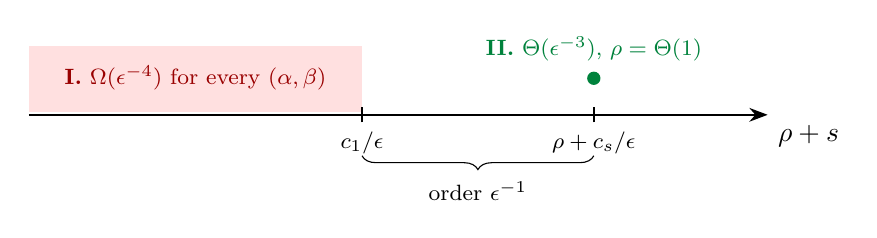
\begin{tikzpicture}[x=0.92cm,y=0.8cm,>=Stealth]
    \draw[->,thick] (0,0) -- (10.2,0) node[below right] {$\rho+s$};
    \fill[red!12] (0,0.05) rectangle (4.6,1.1);
    \node[align=center,red!60!black] at (2.3,0.58)
        {\footnotesize \textbf{I.}\ $\Omega(\epsilon^{-4})$ for every $(\alpha,\beta)$};
    \draw[thick] (4.6,-0.12) -- (4.6,0.12);
    \node[below] at (4.6,-0.12) {\footnotesize $c_1/\epsilon$};
    \draw[thick] (7.8,-0.12) -- (7.8,0.12);
    \node[below] at (7.8,-0.12) {\footnotesize $\rho+c_s/\epsilon$};
    \fill[okgreen] (7.8,0.58) circle (2.4pt);
    \node[align=center,okgreen,above] at (7.8,0.7)
        {\footnotesize \textbf{II.}\ $\Theta(\epsilon^{-3})$, $\rho=\Theta(1)$};
    \draw[decorate,decoration={brace,amplitude=5pt,mirror}] (4.6,-0.65) -- (7.8,-0.65)
        node[midway,below=6pt] {\footnotesize order $\epsilon^{-1}$};
\end{tikzpicture}

\vspace{0.4cm}
\begin{block}{Answer}
\begin{itemize}\setlength{\itemsep}{4pt}
    \item[\red{\textbf{I.}}] \red{\textbf{No}} for $\rho,s=\Theta(1)$: when $\rho+s\le c_1/\epsilon$, the tight complexity of $\calC_\theta$ is \red{$\Theta(\epsilon^{-4})$}.
    \item[\green{\textbf{II.}}] \green{\textbf{Yes}} with large $s$: fixing $\green{\rho=\Theta(1)}$ and taking $\green{s=c_s/\epsilon}$ achieves the tight complexity \green{$\Theta(\epsilon^{-3})$}.
\end{itemize}
\end{block}
\end{frame}

% ---------------------------------------------------------------------
% Slide: Tightness of the family
% \begin{frame}{Tightness of the Algorithm Family}
% \small
% \begin{block}{Proposition 2}
% For fixed $\rho>0$ and $s=c_s/\epsilon$, every $(\alpha,\beta)\in[0,1]^2$ requires at least $\Omega(\epsilon^{-3})$ iterations.
% \end{block}

% \vspace{0.2cm}
% {\centering
% \renewcommand{\arraystretch}{1.25}
% \setlength{\tabcolsep}{4pt}
% \begin{tabular}{@{}cccc@{}}
% \multicolumn{4}{c}{\textbf{Table 4.} Center stepsize and iteration complexity.}\\
% \toprule
% Method & Parameters & $\alpha$ & \makecell{Iteration\\ complexity} \\
% \midrule
% \makecell{$\calC_\theta$\\ \citeb{Corollary 1(a)}} & $\rho+s\le c_1/\epsilon$ & $\epsilon^{2}$ ($\beta=1$) & $\Theta(\epsilon^{-4})$ \\
% \makecell{$\calC_\theta$\\ \citeb{Corollary 1(b), Proposition 2}} & $\rho=\Theta(1)$, $s=c_s/\epsilon$ & $\epsilon$ ($\beta=0$) & $\Theta(\epsilon^{-3})$ \\
% \bottomrule
% \end{tabular}\par}

% \vspace{0.3cm}
% \begin{block}{Answer}
% \centering
% \large Yes, if $s$ is large: $\rho+s$ must be of order $\epsilon^{-1}$, and a large $s$ suffices while $\rho$ stays fixed.
% \end{block}
% \end{frame}

% =====================================================================
\section{Acceleration}
% =====================================================================

% ---------------------------------------------------------------------
\begin{frame}{Open Question: Below $\epsilon^{-3}$}
\small
\begin{block}{Open Question}
\centering
For Problem~(P), what is the optimal iteration complexity of fixed-penalty linearized ALMs?
\end{block}

\vspace{0.35cm}
\centering
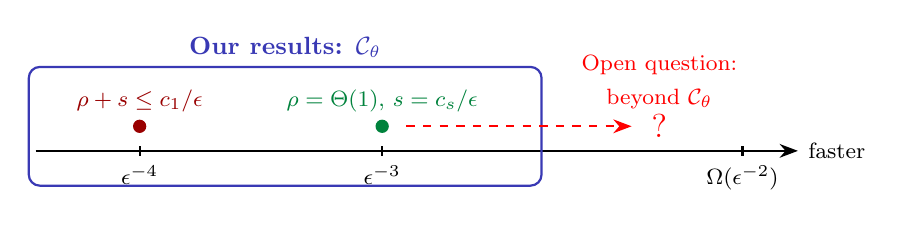
\begin{tikzpicture}[x=0.88cm,y=0.52cm,>=Stealth]
    \draw[->,thick] (0,0) -- (11.0,0) node[right] {\footnotesize faster};
    \draw[thick] (10.2,-0.12) -- (10.2,0.12);
    \node[below] at (10.2,-0.12) {\footnotesize $\Omega(\epsilon^{-2})$};
    \draw[thick] (1.5,-0.12) -- (1.5,0.12);
    \node[below] at (1.5,-0.12) {\footnotesize $\epsilon^{-4}$};
    \draw[thick] (5.0,-0.12) -- (5.0,0.12);
    \node[below] at (5.0,-0.12) {\footnotesize $\epsilon^{-3}$};
    \fill[red!60!black] (1.5,0.6) circle (2.4pt);
    \node[above,red!60!black] at (1.5,0.7) {\footnotesize $\rho+s\le c_1/\epsilon$};
    \fill[okgreen] (5.0,0.6) circle (2.4pt);
    \node[above,okgreen] at (5.0,0.7) {\footnotesize $\rho=\Theta(1)$, $s=c_s/\epsilon$};
    \draw[llxBlockBlue,thick,rounded corners=4pt] (-0.1,-0.85) rectangle (7.3,2.05);
    \node[anchor=south,llxBlockBlue,font=\bfseries] at (3.6,2.05) {\small Our results: $\calC_\theta$};
    \draw[->,dashed,thick,red] (5.35,0.6) -- (8.6,0.6);
    \node[red] at (9.0,0.6) {\large ?};
    \node[above,red,align=center] at (9.0,0.8) {\footnotesize Open question:\\ \footnotesize beyond $\calC_\theta$};
\end{tikzpicture}

\vspace{0.2cm}
\raggedright
\begin{itemize}\setlength{\itemsep}{3pt}
    \item The first-order lower bound for smooth nonconvex problems is $\Omega(\epsilon^{-2})$ \citeb{Carmon et al.\ '20}.
    \item The optimal single-loop complexity for game stationarity of smooth nonconvex--concave problems is $\Theta(\epsilon^{-5/2})$ \citeb{Pan et al.\ '26; Zhang--Xu '26}.
    \item \red{\textbf{Beyond the algorithm class $\calC_\theta$:}} can momentum, extrapolation, or other update rules for $(\bx,\blmbd,\blue{\bz},\blue{\bmu})$ go below $\epsilon^{-3}$?
\end{itemize}
\end{frame}


\begin{frame}{Acceleration Beyond $\calC_\theta$}
\small
\begin{block}{Question}
\centering
How can a fixed-penalty linearized ALM leave $\calC_\theta$ and go below $\red{\epsilon^{-3}}$?
\end{block}

\vspace{0.15cm}
\begin{itemize}\setlength{\itemsep}{6pt}
    \item Dual regularization is a Tikhonov term, making the dual problem $\tfrac{1}{s}$-strongly concave:
    \[
        \max_{\blmbd\in\RR^m}\ \calD_\rho(\bx,\blmbd)-\underbrace{\tfrac{1}{2s}\|\blmbd-\blue{\bmu}\|^2}_{\text{Tikhonov regularization}} .
    \]
    \item The single-loop method reaching $\epsilon^{-5/2}$ uses dual regularization of the same order \citeb{Zhang--Xu '26}. Which updates bring a fixed-penalty linearized ALM from $\epsilon^{-3}$ to $\epsilon^{-5/2}$?
    % \item \textbf{Asymptotic convergence} ($s_k\to\infty$): in monotone problems, with vanishing Tikhonov regularization, the iterates converge to the minimum-norm solution \citeb{Bo\c{t}--Nguyen '26; Chen '26}. Which multiplier does a fixed-penalty linearized ALM select, and how fast?
\end{itemize}
\end{frame}

% ---------------------------------------------------------------------

% Slide: Summary
% \begin{frame}{Takeaway}
% \small
% \vspace{0.4cm}
% \begin{enumerate}\setlength{\itemsep}{10pt}
%     \item \textbf{Combined penalty:} in $\calC_\theta$, the dual regularization $s$ acts as a penalty, and $\rho+s$ is the effective penalty parameter.
%     \item \textbf{Lower bound:} if $\rho+s\le c_1/\epsilon$, the iteration complexity of $\calC_\theta$ is $\Omega(\epsilon^{-4})$.
%     \item \textbf{Fixed penalty:} with $\rho=\Theta(1)$ and $s=c_s/\epsilon$, the iteration complexity of $\calC_\theta$ is $\Theta(\epsilon^{-3})$.
% \end{enumerate}

% \vspace{0.4cm}
% \begin{tcolorbox}[colback=gray!6,colframe=gray!50!black,boxrule=0.4pt,arc=2pt,left=4pt,right=4pt,top=3pt,bottom=3pt]
% \centering
% \red{Open: for Problem~(P), what is the optimal iteration complexity of single-loop ALMs with $\rho=\Theta(1)$?}
% \end{tcolorbox}
% \end{frame}

% ---------------------------------------------------------------------
% Slide: Thank You
\begin{frame}[plain,noframenumbering]
\vfill
\centering
{\Large \blue{Thank you!}}
\vfill
\end{frame}

% ---------------------------------------------------------------------
% Slide: References
\begin{frame}[plain,noframenumbering]\frametitle{References}
\scriptsize
\begin{enumerate}
  \item R. I. Bo\c{t} and D.-K. Nguyen. \emph{The proximal alternating direction method of multipliers in the nonconvex setting: convergence analysis and rates}, Math. Oper. Res., 2020.
  \item M. F. Sahin, A. Eftekhari, A. Alacaoglu, F. Latorre and V. Cevher. \emph{An inexact augmented Lagrangian framework for nonconvex optimization with nonlinear constraints}, NeurIPS, 2019.
  \item Z. Li, P.-Y. Chen, S. Liu, S. Lu and Y. Xu. \emph{Rate-improved inexact augmented Lagrangian method for constrained nonconvex optimization}, AISTATS, 2021.
  \item S. Lu. \emph{A single-loop gradient descent and perturbed ascent algorithm for nonconvex functional constrained optimization}, ICML, 2022.
  \item J. Zhang, P. Xiao, R. Sun and Z.-Q. Luo. \emph{A single-loop smoothed gradient descent-ascent algorithm for nonconvex-concave min-max problems}, NeurIPS, 2020.
  \item T. Zheng, L. Zhu, A. M.-C. So, J. Blanchet and J. Li. \emph{Universal gradient descent ascent method for nonconvex-nonconcave minimax optimization}, NeurIPS, 2023.
  \item J. Li, M. Nagarajan, S. Pan and N. Zhang. \emph{Smoothing meets perturbation: unified and tight analysis for nonconvex-concave minimax optimization}, arXiv:2602.14185, 2026.
  \item S. Pan, T. Zheng and J. Li. \emph{Optimal deterministic first-order oracle complexity for nonconvex-concave minimax optimization}, arXiv:2609.14235, 2026.
  \item M. Zhang and Z. Xu. \emph{Matching multi-loop complexities with a single loop: optimal optimization stationarity and best-known game stationarity in nonconvex--concave minimax optimization}, arXiv:2609.17973, 2026.
  \item R. I. Bo\c{t} and D.-K. Nguyen. \emph{Tikhonov regularization of monotone operator flows not only ensures strong convergence of the trajectories but also speeds up the vanishing of the residuals}, J. Complexity, 94, 2026.
  \item Z. Chen. \emph{A unifying view of anchoring via operator-side Tikhonov regularization}, arXiv:2605.30905, 2026.
\end{enumerate}
\end{frame}

\end{document}
